\section{Soluzione proposta}
Dopo una attenta lettura ai paper, abbiamo impostato le nostre domande di ricerca, in modo da avere ben chiaro in mente l'obiettivo che volevamo prefiggerci di raggiungere con tale progetto. Le domande al quale tale documento cerca di dare risposta sono le seguenti:
\begin{itemize}
  \item All'interno di una rete sociale, come massimizzare il numero di persone che visualizzano una notizia in un numero di step determinato?
  \item Dove è possibile posizionare i Bot che generano i contenuti per massimizzare la diffusione ed eventualmente minimizzare il tempo di diffusione?
  \item \'E possibile distinguere chi è venuto in contatto con una notizia pubblicata da un determinato tipo di utente (Bot o Opinion Leader) e che informazione possiamo ottenere da tali caratteristiche?
\end{itemize}
Abbiamo scelto e ricostruito la rete di partenza (grafo dei follower del presidente del Consiglio Giuseppe Conte) e su di essa sono state eseguite una serie di simulazioni con Soil. Abbiamo inoltre scelto di monitorare le infezioni (da considerarsi come diffusione di notizie) analizzando le differenze tra infetti ed esposti. Abbiamo posto attenzione anche al tipo di infezione: se diretta o indiretta, distinguendo anche da chi proviene tale infezione: da Bot, da Opinion Leader o da un altro utente.
\\
Tale progetto è implementato totalmente in Python attraverso il supporto delle seguenti librerie:
\begin{itemize}
    \item Twint: scraper di dati per Twitter;
    \item Networkx: per la gestione delle reti rappresentate sotto forma di grafi;
    \item Plotly: per la visualizzazione dei grafici finali in modo da avere un riscontro visivo dei risultati;
    \item Soil: per l'implementazione del modello di simulazione multi-agente;
    \item Streamlit: per la costruzione di un'applicazione web che permetta di eseguire ogni fase del nostro studio secondo configurazioni personalizzabili, senza necessariamente dover interagire con un terminale;
    \item Pandas: per la gestione e l'analisi dei dati.
\end{itemize}

Siamo quindi partiti da una serie di assunzioni e ipotesi per poi andare a validarle tramite il modello proposto. Tali assunzioni ci hanno guidato nella parametrizzazione del modello, inserendo le probabilità che più ci sembravano vicine alla realtà e in accordo con la letteratura consultata. Le assunzioni prese in considerazione sono le seguenti:
\begin{itemize}
    \item l'Opinion Leader ha influenza maggiore sulla rete rispetto ai Bot;
    \item i Bot hanno un'influenza più sparsa (ampia);
    \item la probabilità di infezione tra utenti è bassa;
    \item la probabilità che l’utente intraprenda un'azione (retweet, commento...) dopo essere entrato in contatto con la notizia è bassa;
    \item la probabilità di passare da esposto a infetto aumenta di molto solo se molti utenti nel vicinato hanno a loro volta intrapreso un'azione rispetto alla notizia.
\end{itemize}

\subsection{Costruzione dei grafi a partire dall'Opinion Leader}
    Il social network di riferimento per questo studio è Twitter, in particolare è stata scelta la rete sociale dell’attuale Presidente del Consiglio Giuseppe Conte (username: \textit{@GiuseppeConteIT}\cite{twitterGiuseppeConte}) in quanto figura autorevole che, al momento dello studio, conta 752'814 seguaci. 
    
    Twitter offre una serie di API ufficiali per il download di determinati dati, tuttavia questo approccio è limitante in termini di richieste per unità di tempo (nella versione standard, per ottenere la lista dei follower sono permesse 15 richieste ogni 15 minuti), in particolare avendo la necessità di scaricare informazioni riguardanti migliaia di utenti.
    
    Si è così scelto di utilizzare uno scraper per velocizzare il processo, in particolare è stato usato TWINT\cite{Twint} (Twint Intelligence Tool).
    
    Inizialmente lo studio voleva essere basato sulla considerazione della rete sociale avente come fulcro il Presidente del Consiglio Conte ma limitata al secondo livello di profondità (quindi considerando i follower di Conte e i follower dei follower di Conte). Tuttavia questo approccio avrebbe implicato la gestione di milioni di utenti, una situazione al di fuori delle nostre possibilità. Per tali motivi computazionali abbiamo deciso di introdurre un ulteriore vincolo considerando solamente una frazione dei follower di Conte e tutti i rispettivi follower dei follower considerati (nel primo livello). Nel proseguo della relazione, itermini "utenti" e "nodi" verranno utilizzati come sinonimi.
    
    \newpage
    Nel nostro studio sperimentale sono stati definiti 4 grafici basati su frazioni incrementali rispetto ai follower di Conte, limitati sempre a due livelli di profondità. Di seguito vengono presentati i grafi considerati con i rispettivi riferimenti:
    
    \begin{itemize}
        \item grafo basato su 500 follower di Conte e 2 livelli di profondità, per un totale di 38'485 utenti. Riferimento \textbf{500-users};
        \item grafo basato su 1000 follower e 2 livelli di profondità, per un totale di 105'774 utenti. Riferimento \textbf{1000-users};
        \item grafo basato su 1500 follower e 2 livelli di profondità, per un totale di 127'700 utenti. Riferimento \textbf{1500-users};
        \item grafo basato su 2000 follower e 2 livelli di profondità, per un totale di 215'910 utenti. Riferimento \textbf{2000-users};
    \end{itemize}
  
    \'E stata effettuata un'analisi preliminare per verificare che i grafi ottenuti rispettassero effettivamente la proprietà dell'\textit{invarianza di scala}. La tabella \ref{tab:neighbors} mostra la numerosità di nodi rispetto all'ampiezza del proprio vicinato (ovvero con quanti utenti è in relazione l'utente considerato). Come si può notare, in tutti i grafici la maggior parte dei nodi non conta più di 5 vicini.
    
    \begin{table}[H]
        \centering
        \begin{tabular}{l|r|r|r|r}
            \textbf{Numero di vicini} & \textbf{500-users} & \textbf{1000-users} & \textbf{1500-users} & \textbf{2000-users} \\ 
            \hline
            0-5                       & 38'353                   & 105'493                  & 127'327                   & 215'437                   \\
            6-10                      & 41                       & 80                       & 102                       & 122                       \\
            11-20                     & 21                       & 37                       & 50                        & 64                        \\
            21-50                     & 34                       & 54                       & 67                        & 89                        \\
            51-100                    & 13                       & 35                       & 47                        & 58                        \\
            101-250                   & 10                       & 30                       & 45                        & 57                        \\
            251-500                   & 12                       & 21                       & 27                        & 37                        \\
            500+                      & 12                       & 35                       & 46                        & 57                       
        \end{tabular}
        \caption{Numerosità dei nodi rispetto all'ampiezza del vicinato.}
        \label{tab:neighbors}
    \end{table}
    
    Come ulteriore analisi vengono presentate di seguito raffigurazioni grafiche, scalate in modo da visualizzare dati rilevanti, che mettono in relazione il numero di nodi rispetto al numero di relazioni risultandone in una curva esponenziale negativa.
    
    \begin{figure}[!htbp]
        \centering
        \begin{minipage}[b]{0.49\textwidth}
            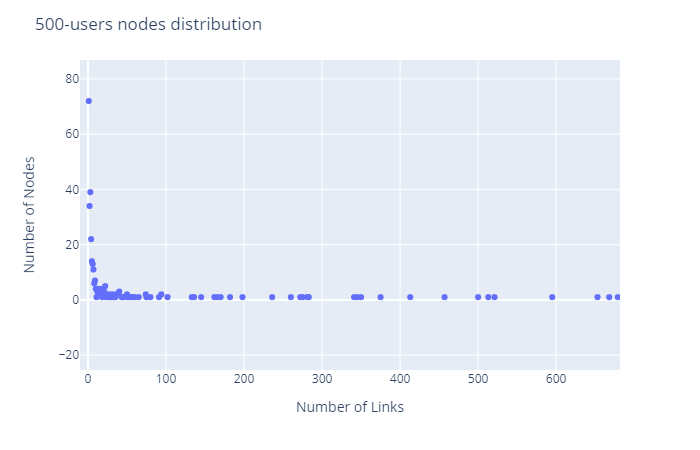
\includegraphics[width=\textwidth]{resources/charts/500_users_nodes.png}
            \caption{Distribuzione nodi grafo 500-users.}
        \end{minipage}
        \hfill
        \begin{minipage}[b]{0.49\textwidth}
            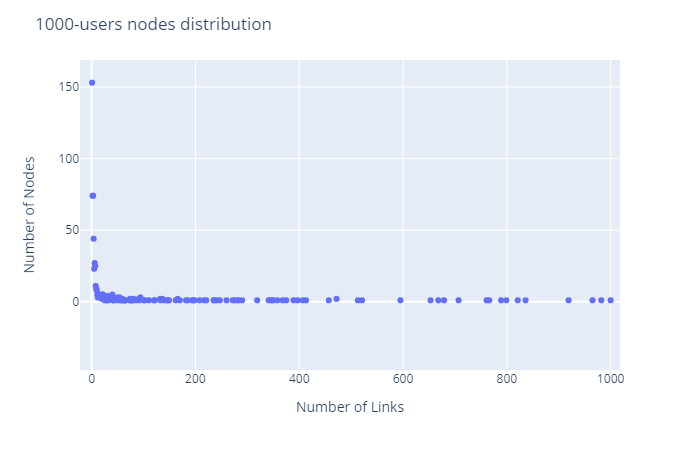
\includegraphics[width=\textwidth]{resources/charts/1000_users_nodes.png}
            \caption{Distribuzione nodi grafo 1000-users.}
        \end{minipage}
    \end{figure}
    
    \begin{figure}[!htbp]
        \centering
        \begin{minipage}[b]{0.49\textwidth}
            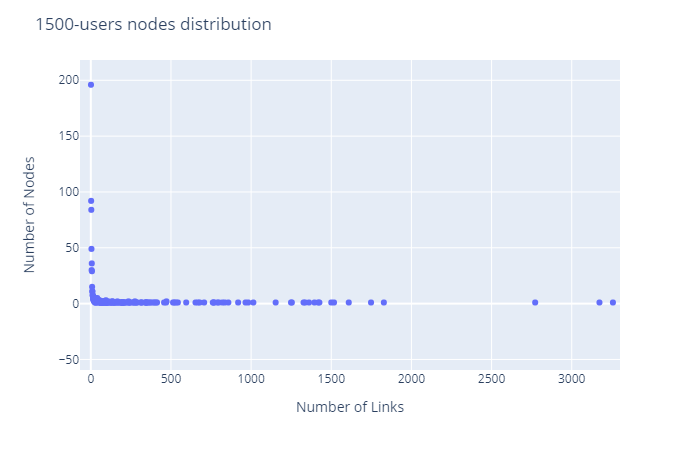
\includegraphics[width=\textwidth]{resources/charts/1500_users_nodes.png}
            \caption{Distribuzione nodi grafo 1500-users.}
        \end{minipage}
        \hfill
        \begin{minipage}[b]{0.49\textwidth}
            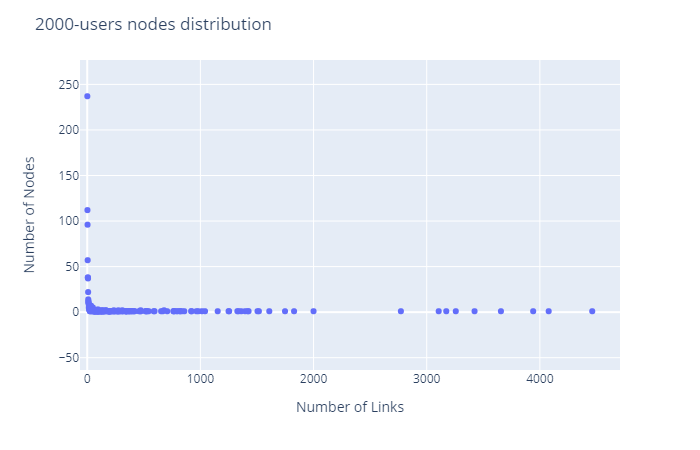
\includegraphics[width=\textwidth]{resources/charts/2000_users_nodes.png}
            \caption{Distribuzione nodi grafo 2000-users.}
        \end{minipage}
    \end{figure}
    
\subsection{Bot}\label{Bot}
    Per determinare la posizione dei Bot all'interno della rete sono state calcolate le principali misure di centralità dei nodi all'interno del grafo.
    \\\\
    \textbf{In-Degree}
    \\
    Rappresenta il numero di archi entranti di un nodo, misura quanto un utente è seguito.\\
    Formalmente: \\
    \begin{center}
        $In-Degree(i) = \displaystyle\sum_{j}x_{ji}$
    \end{center}
    dove: \\
    $x_{ji}$ è un arco diretto dal nodo j al nodo i
    \\
    \\
    \textbf{Betweenness}
    \\
    Rappresenta il numero di volte che un nodo funge da ponte lungo il percorso più breve tra 2 nodi, su una rete sociale corrisponde alla presenza di un utente sui percorsi di comunicazione tra altri utenti.\\
    Formalmente: \newline
    \begin{center}
         $Betweenness(i) = \displaystyle\sum_{j \neq k } g_{jk}(i)/g_{jk}$ 
    \end{center}
    dove: \\
    $g_{jk}$ è il numero di cammini minimi tra i nodi j e k \newline 
    $g_{jk(i)}$ è il numero di cammini minimi tra i nodi j e k passanti per il nodo i
   \\
    \\
    \textbf{Autovettori}
    \\
    Misura l'importanza di un nodo, un nodo è considerato tale se puntato da altri nodi importanti. \\
    Formalmente: \\
    \begin{center}
    $EigenvectorCentrality(i) = \frac{1}{\lambda}\displaystyle\sum_{k}a_{k,i}x_{k}$
    \end{center}
    dove: \\
    $A=(a_{i,j})$ è la matrice di adiacenza del grafo.
\\\\
    É stata inoltre, svolta una simulazione considerando una posizione randomica dei Bot.

\subsection{Simulazioni}
    Durante le simulazioni è stato selezionato come Opinion Leader l’esatto nodo che, all’interno del grafo ottenuto grazie allo scraper, rappresenta il Presidente del Consiglio. I Bot all’interno delle simulazioni sono sempre 10 tuttavia differiscono per la loro posizione all’interno della rete. Poiché gli stessi nodi con in-degree maggiore sono gli stessi con betweenness maggiore allora la simulazione sarà unica. Si avranno quindi tre simulazioni:
    \begin{itemize}
    \item Simulation\_BTW: simulazione nella quale i Bot sono stati posizionati sui nodi aventi betweenness maggiore.
    \item Simulation\_Eigenvector: simulazione nella quale i nodi selezionati come Bot sono i 10 nodi considerati più influenti sulla base degli eigenvector score.
    \item Simulation\_Random: simulazione nella quale i nodi selezionati come Bot sono presi in modo randomico.
    \end{itemize}
    \subsection{Configurazione di SOIL}\label{ConfigSoil}

        \subsubsection{Definizione del modello}
        Il modello è stato sviluppato in un file python contenente la definizione dei singoli agenti che verranno impiegati nella fase di simulazione in accordo con le direttive specificate nel file YML. Per ogni agente viene quindi creata una classe la quale avrà degli stati e dei metodi che ne descrivono i comportamenti e le interazioni tra i vari agenti. In questo caso  di studio sono state definite 3 tipologie di agenti, ispirate al modello epidemiologico SEI (Suscettibile, Esposto, Infetto):
        \begin{itemize}
            \item OpinionLeader: è l’utente a partire dal quale è stato generato il grafo, nel nostro caso rappresenta il Presidente del Consiglio.
            \item Bot: sono gli agenti interessati a far espandere una notizia pubblicandone contenuti inerenti, hanno quindi un potere di influenza mediamente alto. La selezione di queste entità è stata effettuata sulla base dell'analisi dei grafi come descritto nella sezione \ref{Bot}.
            \item User: rappresentano gli utenti comuni e possono trovarsi in tre stati:
                  \begin{itemize}
                      \item Non esposto: l’utente non è entrato in contatto con una determinata notizia; non ne è  stato esposto da altri utenti, nè guardando la Home di Twitter o cercando manualmente (quest'ultima casistica è gestita dal campo "prob\_search\_spread").
                      \item Esposto: l’utente è entrato in contatto con la notizia ma non ha ancora intrapreso alcuna azione.
                      \item Infetto: l’utente non solo è stato esposto ma ha anche palesato il suo interesse verso la notizia effettuando un'azione, rendendosi potenziale fonte di esposizione verso altri utenti.
              \end{itemize}
        \end{itemize}
        
        All’inizio della simulazione i nodi che rappresentano l'Opinion Leader e i Bot sono considerati fonte di diffusione dell'informazione. Sono stati inizializzati impostandone lo stato ad "infetto". 
        
        Per una questione di maggior controllo dei risultati finali, e quindi per vedere chi e quanto ha contribuito alla propagazione dell'informazione, è stato introdotto un parametro \textit{type}. Quest’ultimo assume valore 1 nel caso la propagazione sia partita dall’Opinion Leader; 2 nel caso avvenga dai Bot. Notasi che gli utenti infettati da altri utenti propagano comunque il tipo da cui sono stati infettati, e quindi ad esempio un utente infettato da un utente che era stato in principio infettato da un Bot avrà tipo 2 e sarà quindi conteggiato come infettato da Bot.
        
        \subsubsection{File YML}
        Il file YML racchiude le specifiche delle simulazioni che caratterizzano l'esecuzione tramite Soil.
        
        Tra i parametri personalizzabili specificati elenchiamo:
        \begin{itemize}
          \item max\_time: numero di step effettuati nella simulazione.
          \item num\_trials: parametro tramite il quale si può decidere se ripetere la stessa simulazione più volte indicando il numero di volte che sarà eseguita.
          \item network\_params: parametro che permette di specificare il grafo su cui sarà effettuata la simulazione.
          \item states: parametro che permette di personalizzare il singolo nodo tramite il suo identificativo. Ciò ci ha permesso di mantenere fissa la posizione di Conte e di verificare come i risultati delle simulazioni variassero in relazione alla specifica posizione dei Bot. 
        \end{itemize}

    \subsection{Web app}
      Per ragioni di riproducibilità più agevole e per estensibilità è stato scelto di sviluppare una web app che permettesse l’esecuzione di tutte le fasi contemplate dall’applicativo e di presentare i risultati in forma di grafici.
      
      Per lo sviluppo di qeusta interfaccia è stata usata la libreria Streamlit. Streamlit è un framework open-source particolarmente utile per data scientists e sviluppatori che lavorano nel campo di machine learning.\\

      Di seguito si illustrano le varie fasi dell’app.
        \subsubsection{Fasi dell'app}
          
          \textbf{Download dati da Twitter}
          \\
          In questa fase abbiamo utilizzato lo scraper TWINT per ottenere i followers di Conte e, a loro volta, i followers dei followers di Conte. Il risultato ottenuto è un file .csv per ogni utente di Twitter, all'interno del quale sono segnati gli user dei followers.
          \\
          \textbf{Creazione del grafo}
          \\
          Da questi file .csv ottenuti dalla fase precedente, si è creato il grafo orientato (secondo la relazione di “Follow”) tramite la libreria NetworkX.
          \\
          \textbf{Posizionamento Bot e simulazione SOIL}
          \\
          Oltre a configurare e far eseguire le simulazioni di soil, così come spiegato nella sezione \ref{ConfigSoil}, in tale fase sono state effettuate le principali misure di centralità dei nodi nel grafo in modo da determinare la posizione dei Bot, ed effettuate le simulazioni appropriate.
          \\
          \textbf{Visualizzazione grafo risultante}
          \\
          In questa fase vengono mostrati i risultati delle simulazioni in forma di grafo. I nodi del grafo sono stati colorati differentemente a seconda dello stato dell’agente corrispondente (non esposto, esposto, infetto), inoltre viene riportato anche il tipo di nodo che ha causato la diffusione/contagio.
          \\
          \textbf{Statistiche sulla diffusione}
          \\
          A questo punto abbiamo provveduto a calcolare le statistiche ottenute dai risultati, andando a computare le percentuali dei non esposti, esposti, infetti, per ogni fase e le rispettive fonti di diffusione (Opinion Leader, Bot, User).
        \subsubsection{Uso di Streamlit}
          L'applicazione web dispone di un pannello di configurazione tramite il quale è possibile configurare ed eseguire ogni singola fase.
          
          \begin{figure}[H]
              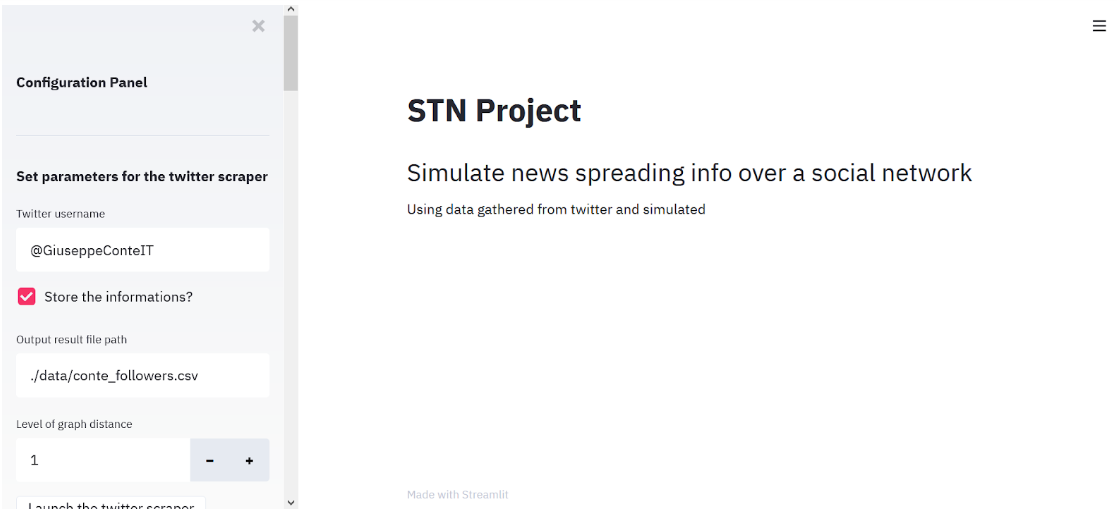
\includegraphics[width=16cm]{resources/panelApp.png}
              \caption{Visualizzazione dell'applicazione web.}
          \end{figure}
          
          Da tale pannello è possibile configurare i seguenti parametri:
          \begin{itemize}
          
            \item Parametri per il Twitter scraper:
              \begin{itemize}
                \item Scelta dell'username dell'account su cui avviare lo scraper.
                \item Salvataggio dei dati in formato csv.
                \item Selezione del percorso nel quale salvare il file csv contenente i follower dell'account indicato.
                \item Specificare a che livello scendere nel grafo dei follower (1 o 2).
              \end{itemize}
              
            \item Parametri per generare il grafo:
              \begin{itemize}
                \item Selezione del percorso da cui prendere le informazioni (csv) sui follower.
                \item Selezione la cartella da cui prendere il secondo livello del grafo (se presente).
                \item Scegliere il nome del grafo.
                \item Selezionare se salvare il grafo come diretto o non diretto.
                \item Numero di follower da considerare.
              \end{itemize}
              
            \item Parametri per la selezione dei Bot:
              \begin{itemize}
                \item Percorso in cui si trova il grafo  da utilizzare.
                \item Selezione della misura di centralità da calcolare.
                \item Selezione del numero di Bot da inserire nella rete.
              \end{itemize}
              
            \item Parametri per la simulazione tramite Soil:
              \begin{itemize}
                \item Percorso in cui si trova il file YML da utilizzare per configurare la simulazione.
                \item Selezione del nome della simulazione.
                \item Selezione del percorso in cui si trova la cartella principale dedicata alle simulazioni.
                \item Inserimento del numero massimo di iterazioni della simulazione.
                \item Inserimento del numero di volte che la simulazione sarà eseguita.
                \item Selezione del grafo da utilizzare come topologia.
              \end{itemize}
              
            \item Parametri per la visualizzaione dei grafici  risultanti:
              \begin{itemize}
                \item Selezione del grafo da utilizzare.
                \item File csv contenente l’output della simulazione di Soil.
                \item Nome della simulazione, sulla base della tipologia di selezione dei Bot (Random, Betweenness o Eigenvector).
                \item Numero di step effettuati durante la simulazione sul grafo.
                \item Indicare se visualizzare o meno il grafo (per una questione di performance).
              \end{itemize}
              
            \item Parametri per calcolare le statistiche finali:
              \begin{itemize}
                \item Nome della simulazione, sulla base della tipologia di selezione dei Bot (Random, Betweenness o Eigenvector).
                \item Numero di step effettuati durante la simulazione sul grafo.
              \end{itemize}
          \end{itemize}